\clearpage
\newgeometry{left=-0.50cm,right=-0.50cm,top=0cm,bottom=0cm,centering}
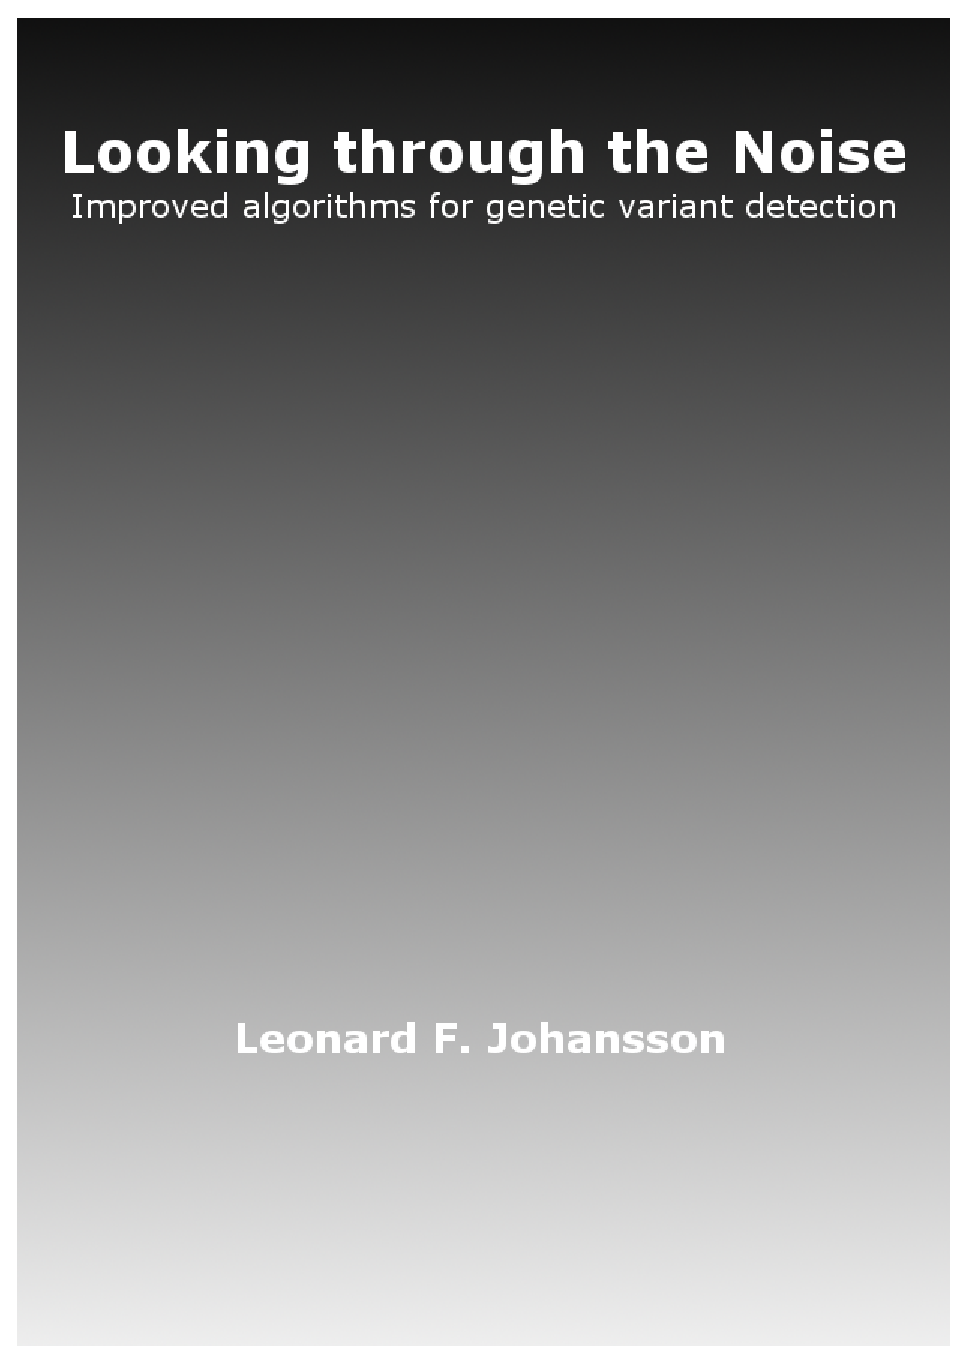
\includegraphics[width=0.935\textwidth,height=1.0\textheight]{img/frontcover_zw}
\restoregeometry
\clearpage

{\small
	\noindent
	Leonard Fredericus Johansson. \textbf{Looking through the noise: novel algorithms for genetic variant detection.} Thesis, University of Groningen, with summary in English and Dutch.
	\\~\\
	Printing of this thesis was financially supported by Rijksuniversiteit Groningen, University Medical Center Groningen. 
	\\~\\
	Cover design and layout by L.F. Johansson.
	The front cover shows a variant that can only be seen when looking through the noise created by the four DNA nucleotides A, C, G and T. 
	\\~\\
	Printed by Ipskamp Drukkers, Enschede.\\
	\\
	© 2019 L.F. Johansson. All rights reserved. No part of this book may be reproduced or transmitted in any form or by any means without permission of the author.\\
	\\
	ISBN: XXX-XX-XXX-XXXX-X \mbox{~~~~~} ISBN (electronic version): 978-94-034-1857-5
}

\begin{figure}[!htbp]
	\centering
	
	\begin{minipage}[b]{0.24\textwidth}
		
\includegraphics[width=\textwidth]{img/colofon_umcg_zw}
	\end{minipage}
	\hfill
	\begin{minipage}[b]{0.29\textwidth}
		\raisebox{0.4\height}{
\includegraphics[width=\textwidth]{img/colofon_rug_zw}}
	\end{minipage}
	 \hfill
	\begin{minipage}[b]{0.23\textwidth}
		\raisebox{0.25\height}{
\includegraphics[width=\textwidth]{img/colofon_fsc_zw}}
	\end{minipage}
\end{figure}

\clearpage

\begin{flushleft}
	
\includegraphics[scale=0.8]{img/rugr_logoen_zwart_rgb}
\end{flushleft}

\begin{center}
	\linespread{1.00} % squish slightly to fit everyone on page
	~\\
	\huge
	\textbf{Looking through the noise}
	\\~\\
	\large
	improved algorithms for genetic variant detection
	\\~\\
	\linespread{1.05} % and back to normal
	
	
	\large
	\textbf{PhD thesis}
	\\~\\
	\normalsize
	to obtain the degree of PhD at the\\
	University of Groningen\\
	on the authority of the\\
	Rector Magnificus prof. C. Wijmenga\\
	and in accordance with \\
	the decision by the College of Deans.
	\\~\\
	This thesis will be defended in public on
	\\~\\
	Wednesday 25 September 2019 om 12.45 hours 
	\\~\\~\\
	by
	\\~\\~\\
	\large
	\textbf{Leonard Fredericus Johansson}
	\\~\\
	\normalsize
	born on 29 May 1980\\
	in Hefshuizen\\
	\normalsize
\end{center}

\clearpage

\noindent
\textbf{Supervisors}\\
Prof. R.H. Sijmons \\
Prof. M.A. Swertz \\

\noindent
\textbf{Co-supervisor}\\
Dr. B. Sikkema-Raddatz \\

\noindent
\textbf{Assessment Committee}\\
Prof. V.V.A.M. Knoers\\
Prof. M. Vihinen\\
Prof. J.K. Ploos van Amstel\\


\clearpage

\noindent
\textbf{Paranymphs}\\
E.N. de Boer\\
K.K. van Dijk-Bos\\

\clearpage
\null\newpage

\noindent
	\Large
Propositions

\small

\begin{enumerate}
	
	\item Depending on how samples are prepared and analyzed, next-generation sequencing is suitable for detection of both base-level variants and structural variants. \textsl{(this thesis)}
	
	\item High coverage next-generation sequencing data is suitable for single-exon copy number variation detection. \textsl{(this thesis)}
	
	\item Before biological variability can be detected in next-generation sequencing, first laboratory induced variability has to be minimalized \textsl{(this thesis)}
	
	\item International screening program criteria  are currently not fully met for opportunistic genetic screening.\textsl{(this thesis)}
	
	\item In non-invasive prenatal testing, the use of multiple independent models increases the reliability of  the prediction of presence of a trisomy from a single data set. \textsl{(this thesis)}
	
	\item The same measurement outcome in non-invasive prenatal testing gives different results for women with different prior risks of carrying a child with a trisomy. \textsl{(this thesis)}
	
	\item Noise is everything that, from a certain perspective, blocks the path between reality and measurement outcome. \textsl{(this thesis)}
	
	\item Data can be of high and low quality at the same time (depending on what information should be retrieved from the data). \textsl{(this thesis)}
	
	\item Understanding how or why is seldom as useful as understanding that things are. \textsl{(Robin Hobb, Fool's Assassin)}
	
	\item It’s not what you look at that matters, it’s what you see. \textsl{(Henry David Thoreau)}
	
\end{enumerate}
